\documentclass{article}
\usepackage[T1]{fontenc}
\usepackage{lmodern}
\usepackage{graphicx}
\usepackage{amsmath,amssymb}
\usepackage[a4paper,margin=2cm]{geometry}
\usepackage[absolute,overlay]{textpos}
\setlength{\TPHorizModule}{1mm}
\setlength{\TPVertModule}{1mm}
\usepackage[indonesian]{babel}
\usepackage{hyperref}
\setlength{\emergencystretch}{2em}
% unit: Halaman 46

\begin{document}

% === Halaman 46 (llm) ===

\vspace{175.23mm}

Sumber: William Stalling, Cryptography and Network Security\nOverview & Chapter 1\n\vspace{60mm}\n\textbf{\Large Active Attack: Fabrication}

% deskripsi: Diagram ilustrasi serangan aktif berupa fabrikasi pesan, menunjukkan penyerang (Darth) yang mengirimkan pesan palsu ke Alice melalui internet, menginterupsi komunikasi antara Bob dan Alice.
% bbox normalisasi: [0.1900, 0.1700, 0.8300, 0.7600]
\begin{textblock*}{134.40mm}(39.90mm,50.49mm)
\noindent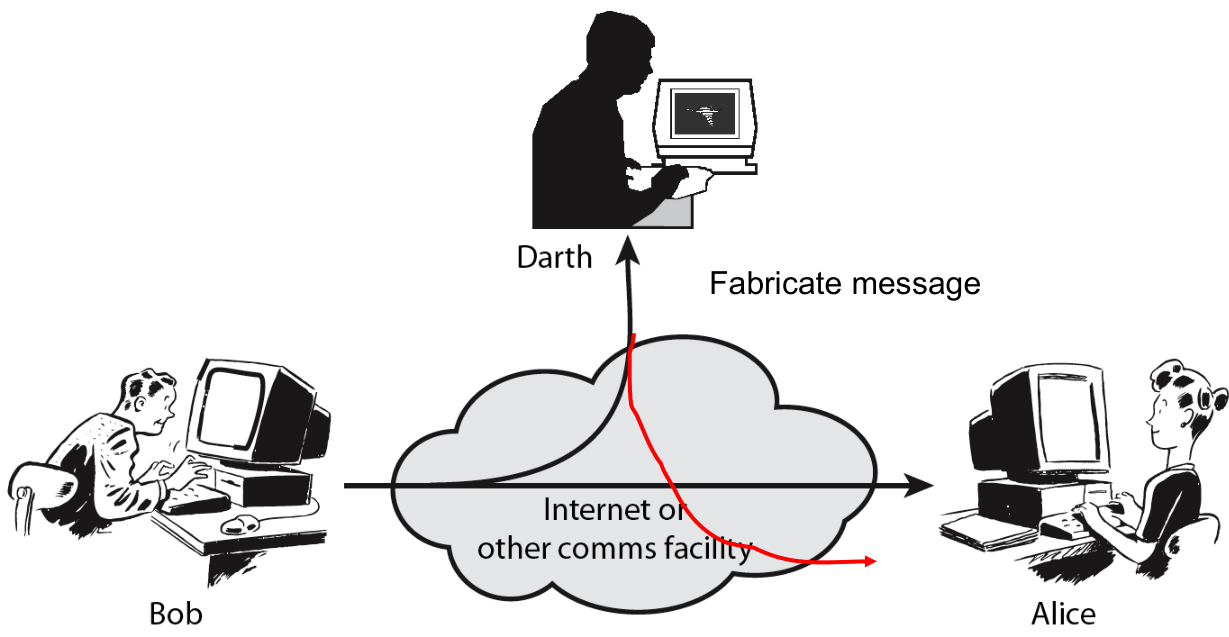
\includegraphics[width=134.40mm,height=175.23mm]{../../images/llm/page_046_img_01.png}%
\end{textblock*}

\end{document}
